\documentclass[../Interim_Report_Master]{subfiles}
\begin{document}
\hypertarget{res}{\section{Results}\label{res}}
\subsection{Probability Density Functions of the Temporal Evolution of Temperature and Mass }
The code is setup so the initial temperature and mass is the same for all the droplets. In the case of no convective heat transfer it would be expected that all droplets evaporate at the same rate and have the same increase in temperature. However, placing the droplets in a Taylor-Green vortex means the droplets will experience different fluid velocities. Therefore there will be a range of convective heat transfer across the droplets.

This effect can be observed by plotting how the probability density function (PDF) evolves over time. The spread of droplet temperature can be plotted by using the deviation ${T_d}'$:
\begin{equation}
{T_d}' = T_d - \bar{T_d}
\end{equation}

This process can be used at each timestep to produce a 3D PDF to show how the deviation of droplet temperatures changes.
\begin{table}[h]
	\centering
	\begin{tabular}{|l c|}
		\hline
		\large{\textbf{Parameter}} & \large{\textbf{Setting}} \\ \hline
		\textbf{Droplet Properties} &  \\
		Molecular Weight of Vapour Phase $W_V$ & $18.015~kg/kg~mol$ \\ 
		Boiling Temperature $T_B$ & $373.15~K$ \\ 
		Density of Liquid Phase $\rho_L$ & $997~kg/m^3$ \\
		Specific Heat Capacity of Liquid Phase $C_L$ & $4184~J/(kg~K)$ \\ 
		Initial Temperature $T_{d0}$ & $282~K$ \\ 
		Initial Diameter $D_0$ & $\sqrt{1.1}~mm$ \\ \hline 
		\textbf{Gas Properties} &  \\ 
		Molecular Weight of Phase $W_C$ & $28.97~kg/(kg~mol)$ \\ 
		Temperature $T_G$ & $298~K$ \\
		Density $\rho_G$ & $1.184~kg~m^{-3}$ \\ 
		Specific Heat for Constant Pressure $C_{P,G}$ & $1007~J~kg~K$ \\
		Free Stream Vapour Mass Fraction $Y_G$ & $0$ \\ \hline
		\textbf{Atmospheric Properties} &  \\ 
		Pressure $P_{atm}$ & $101325~Pa$ \\ \hline 
		\textbf{Fluid Conditions} & \\
		Flow Magnitude $A$ & $0.05$ \\
		Vortex Frequency $a$ & $3$ \\ \hline
		\textbf{Physical Constants} & \\
		Gravity $g$ & $0~ms^{-1}$ \\ 
		Gas Constant $\bar{R}$ & $8314.5~J/(K(kg~mol))$ \\ 
		Universal Gas Constant $R$ & $287~J/(kg~K)$ \\ \hline
		\textbf{Simulation Settings} & \\
		Correction factor $f_2$ & 1 \\
		Driving Potential $H_{\Delta T}$ & 0 \\ 
		Number of Droplets & 10000 \\ 
		Simulation Length & $200\tau_{d,0}$ \\
		Timestep Size $\Delta t$ & $\tau_{d,0}/8$ \\ \hline
	\end{tabular}
	\caption{Simulation settings used for creating the heat and mass PDFs.}
	\label{tab:sim_set}
\end{table}

The simulation was run using the settings in Table \ref{tab:sim_set}. Note there is no gravitational acceleration, so only the effects of the flow are considered. Including a weight force would induce an effect known as enhanced settling. All further necessary values are calculated as per Sections 4.4.1 and 4.4.2. The corresponding PDF for the droplet temperature evolution is shown in Figure \ref{temp_pdf}.
\begin{figure}[h]
\centering %test2
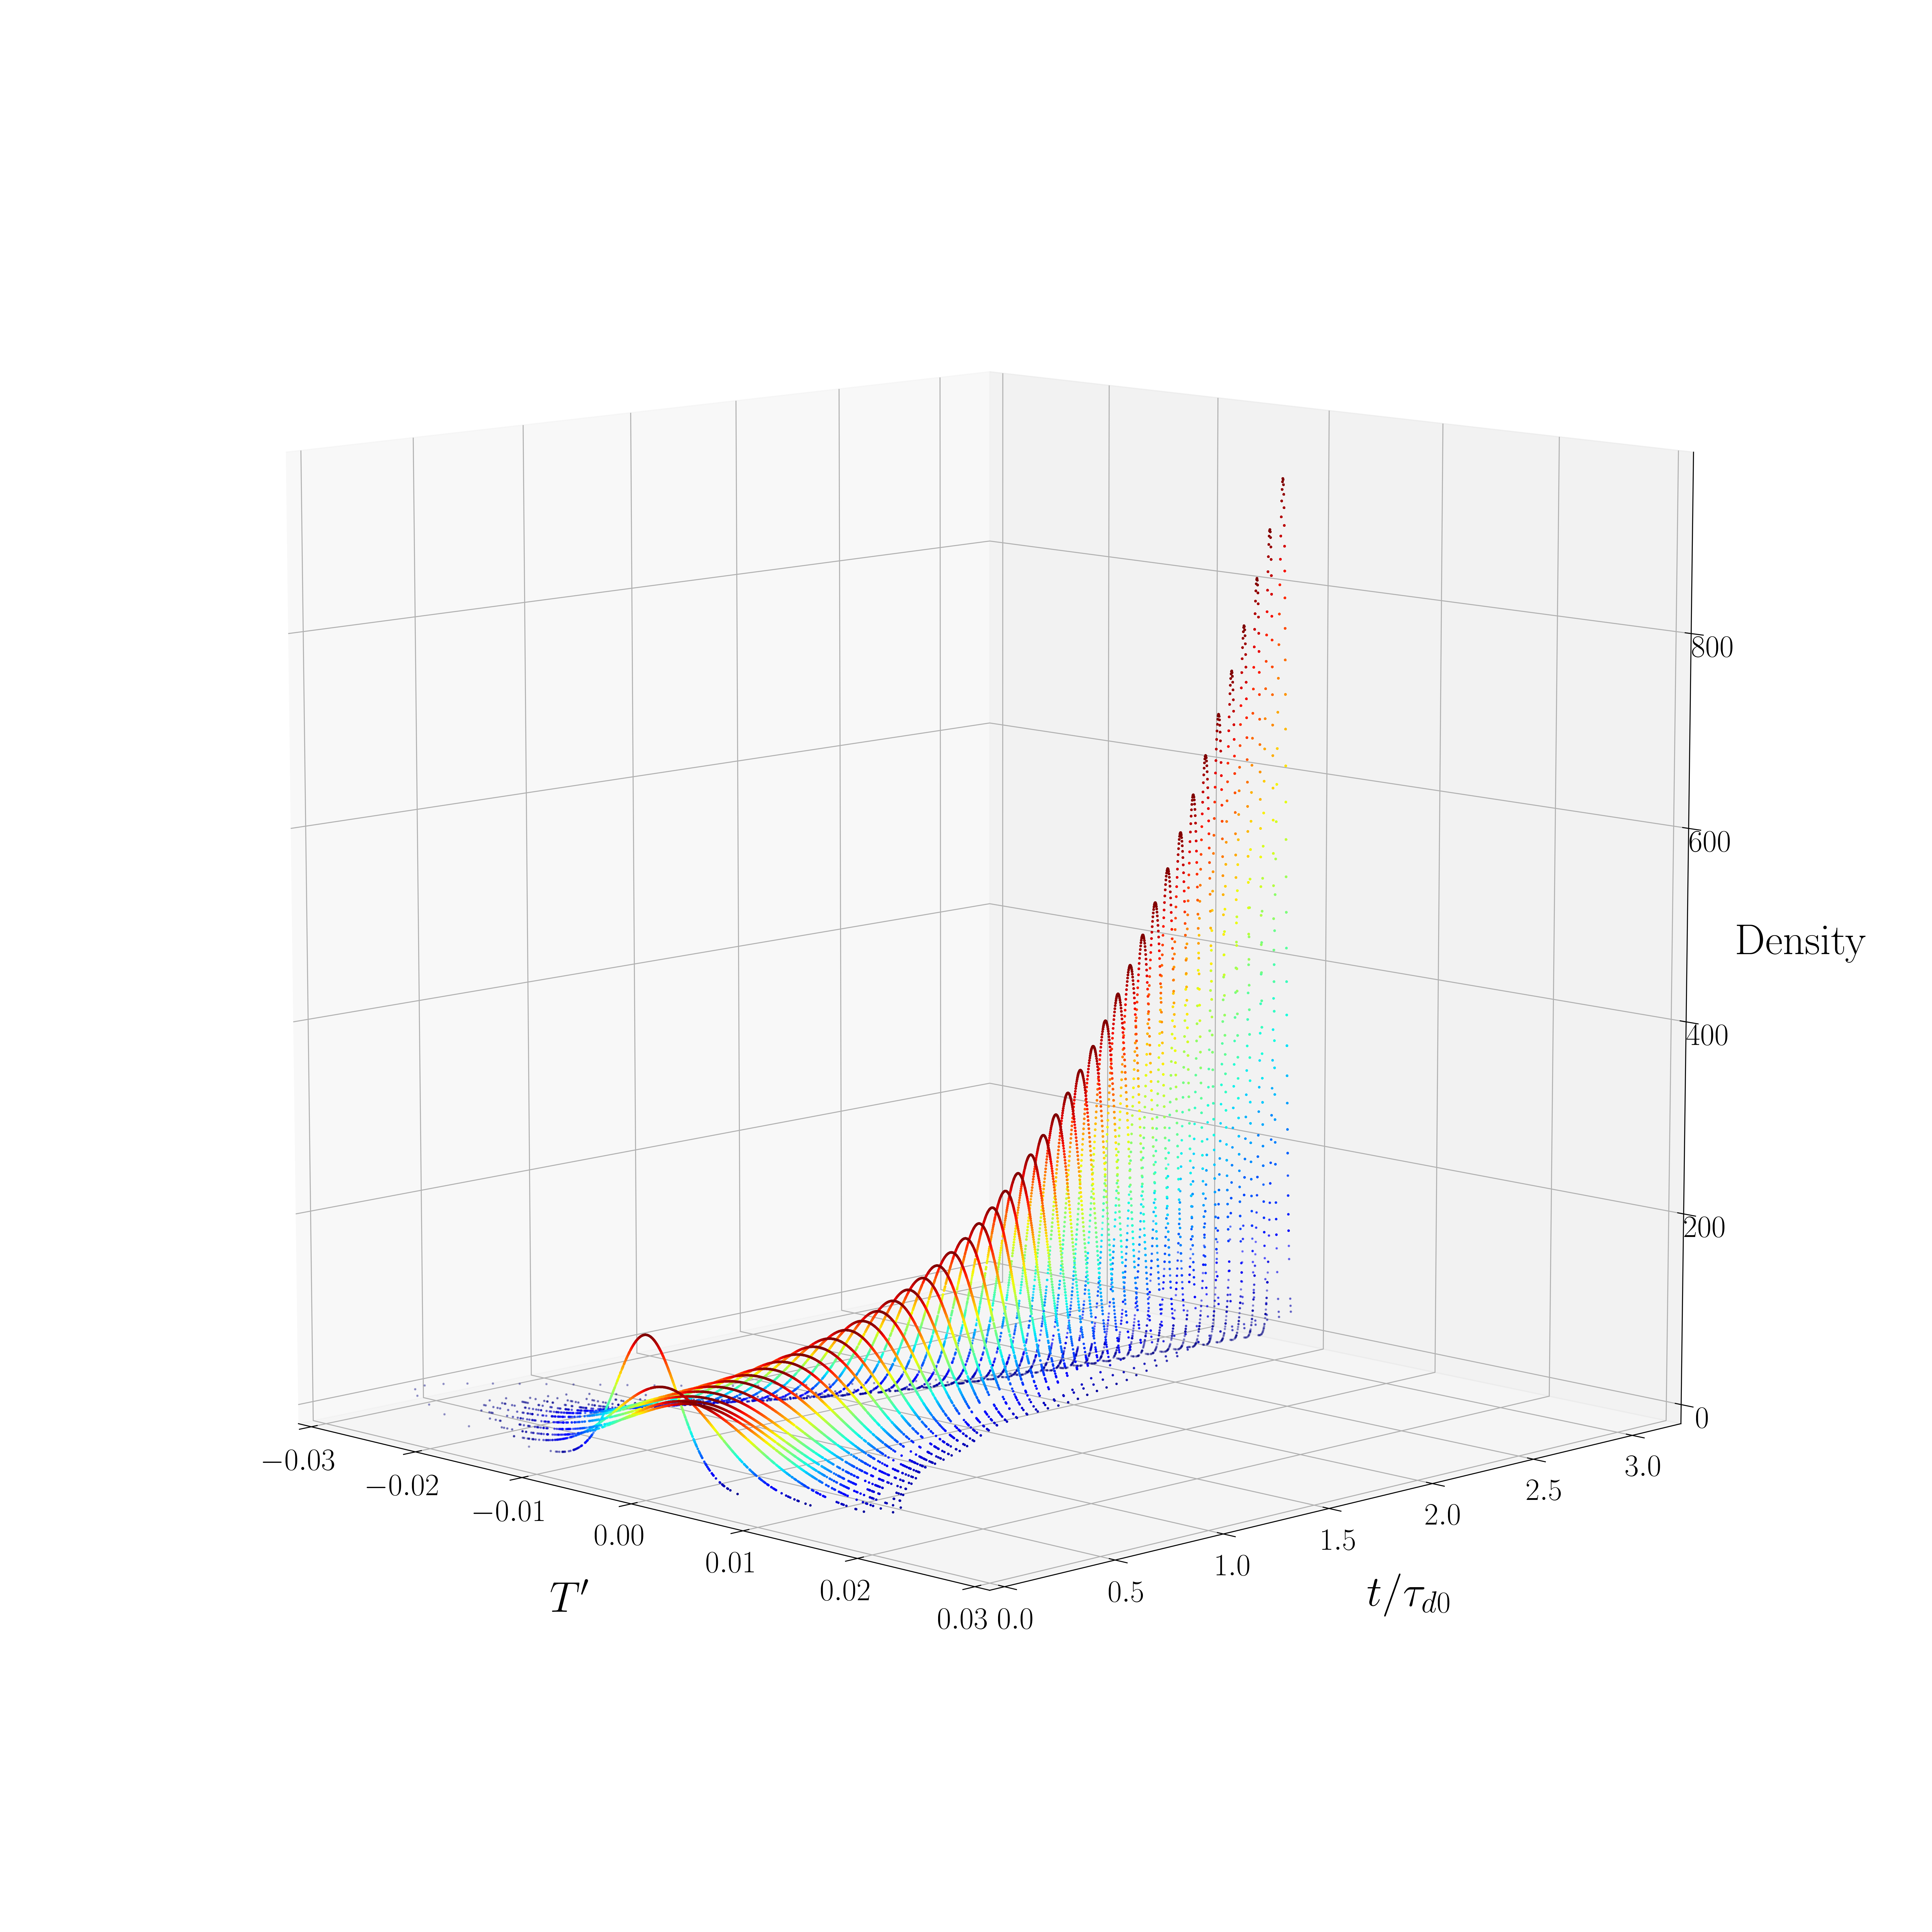
\includegraphics[width=\textwidth, trim={0.8in 3in 0.5in 4in}, clip]{./Diagrams/Temperature_PDFs.png}
\caption{PDFs of the droplet temperature deviation for the first 50 timesteps of the simulation.}
\label{temp_pdf}
\end{figure}

The initial conditions are not shown in this plot but would be a Dirac delta function centered around zero on the x-axis with a density of 10000. For the next 5 timesteps the deviation of droplet temperature increases as the droplets spread out into the fluid. The deviation then begins to decrease as the mean droplet temperature reaches the steady state temperature. 

A similar PDF can be plotted for droplet diameter, much like the temperature deviation the droplet diameter normalised with initial diameter will deviate as the droplets evaporate at different rates. Furthermore, unlike the Figure \ref{temp_pdf} the mean value of the normalised $D^2$ PDF decreases as a result of the droplets losing mass. This is is shown in Figure \ref{diameter_pdf}. 
\begin{figure}[H]
	\centering %Figure_2
	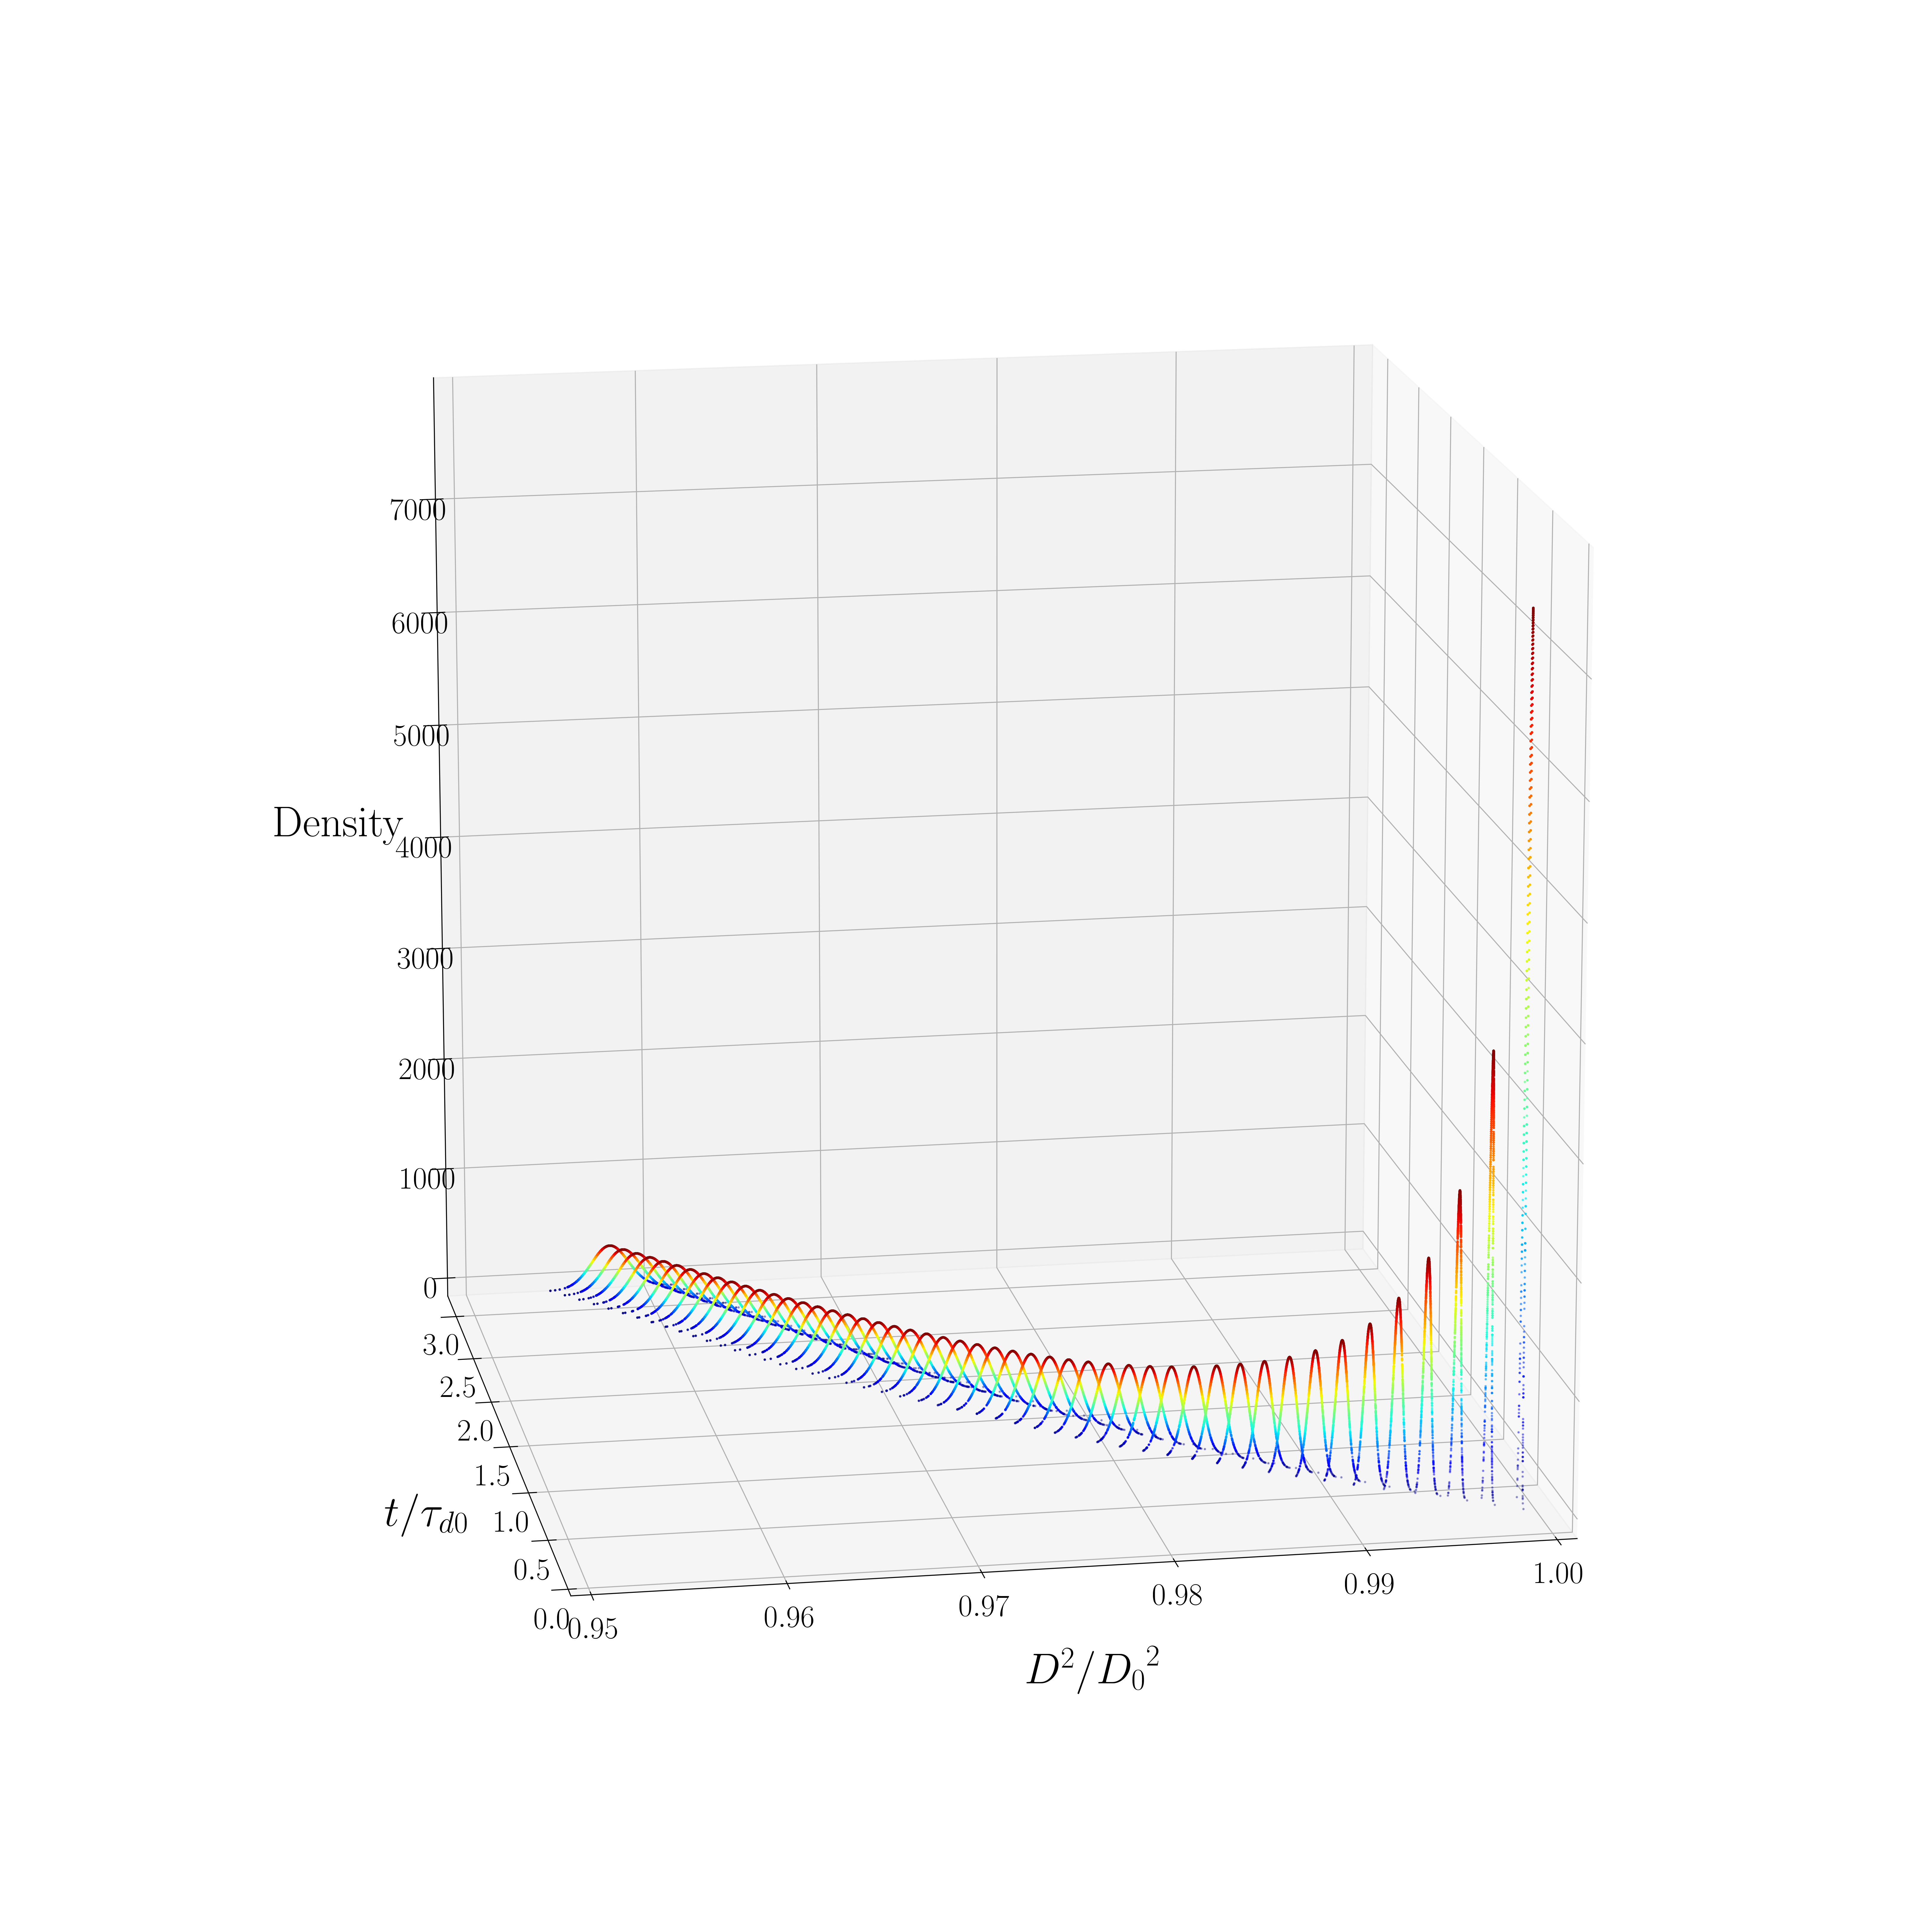
\includegraphics[width=\textwidth, trim={0.8in 2in 0.5in 4in}, clip]{./Diagrams/Mass_PDFs.png}
	\caption{PDFs of the droplet $D^2/{D_0}^2$ for the first 50 timesteps of the simulation.}
	\label{diameter_pdf}
\end{figure}

The relation between droplet mass deviation and droplet temperature deviation is shown in Figure \ref{fig:heat_mass_pdf}. For Figure \ref{fig:heat_mass_pdf}(a) It can be seen that near the start of the simulation the relation between ${T_d}'$ and $D^2/{D_0}^2$ is almost proportional . However, further into the simulation the deviation increases as can be seen in Figure \ref{fig:heat_mass_pdf}(b). Although once the droplets reach an equilibrium temperature the spread of ${T_d}'$ while the deviation in $D^2/{D_0}^2$ has continued to increase as in Figure \ref{fig:heat_mass_pdf}(c).
\begin{figure}[H]
	\centering
	\begin{subfigure}{\textwidth}
		\centering
		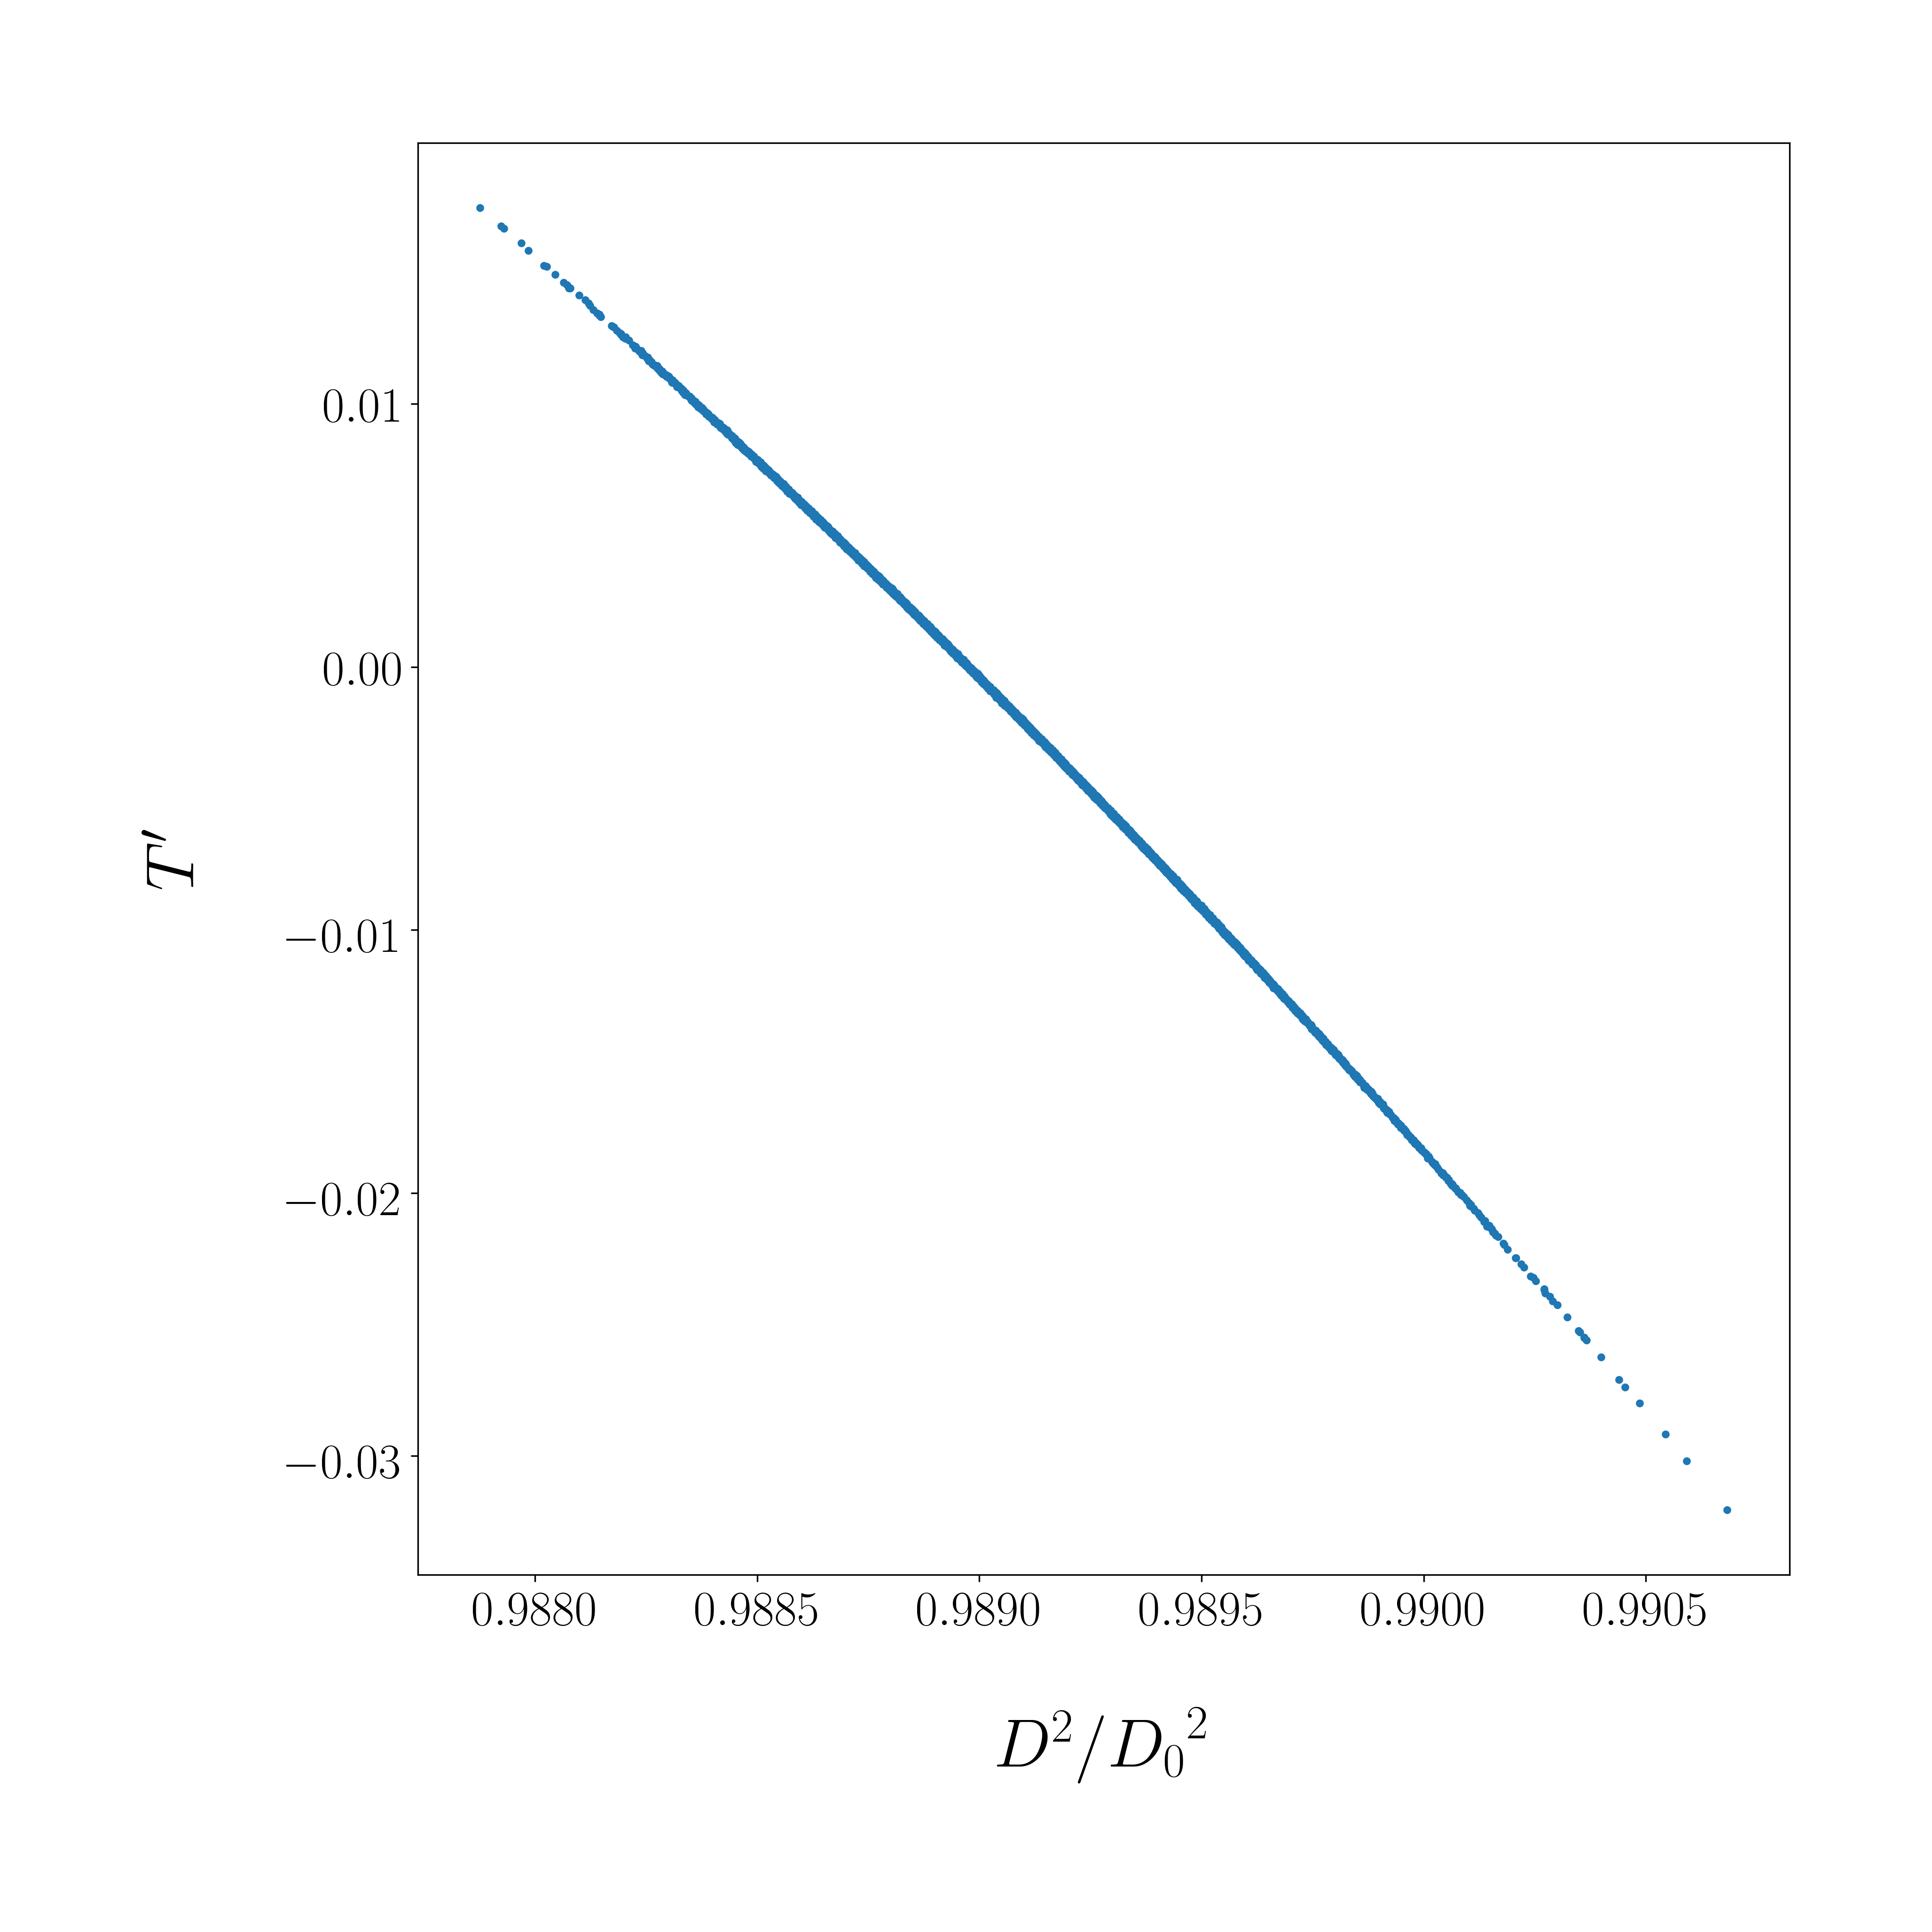
\includegraphics[width=0.7\textwidth]{./Diagrams/Temp_Mass_PDFs_timestep_8.png}
		\caption{}
	\end{subfigure}
\end{figure}
\begin{figure}\ContinuedFloat
	\centering
	\begin{subfigure}{\textwidth}
		\centering
		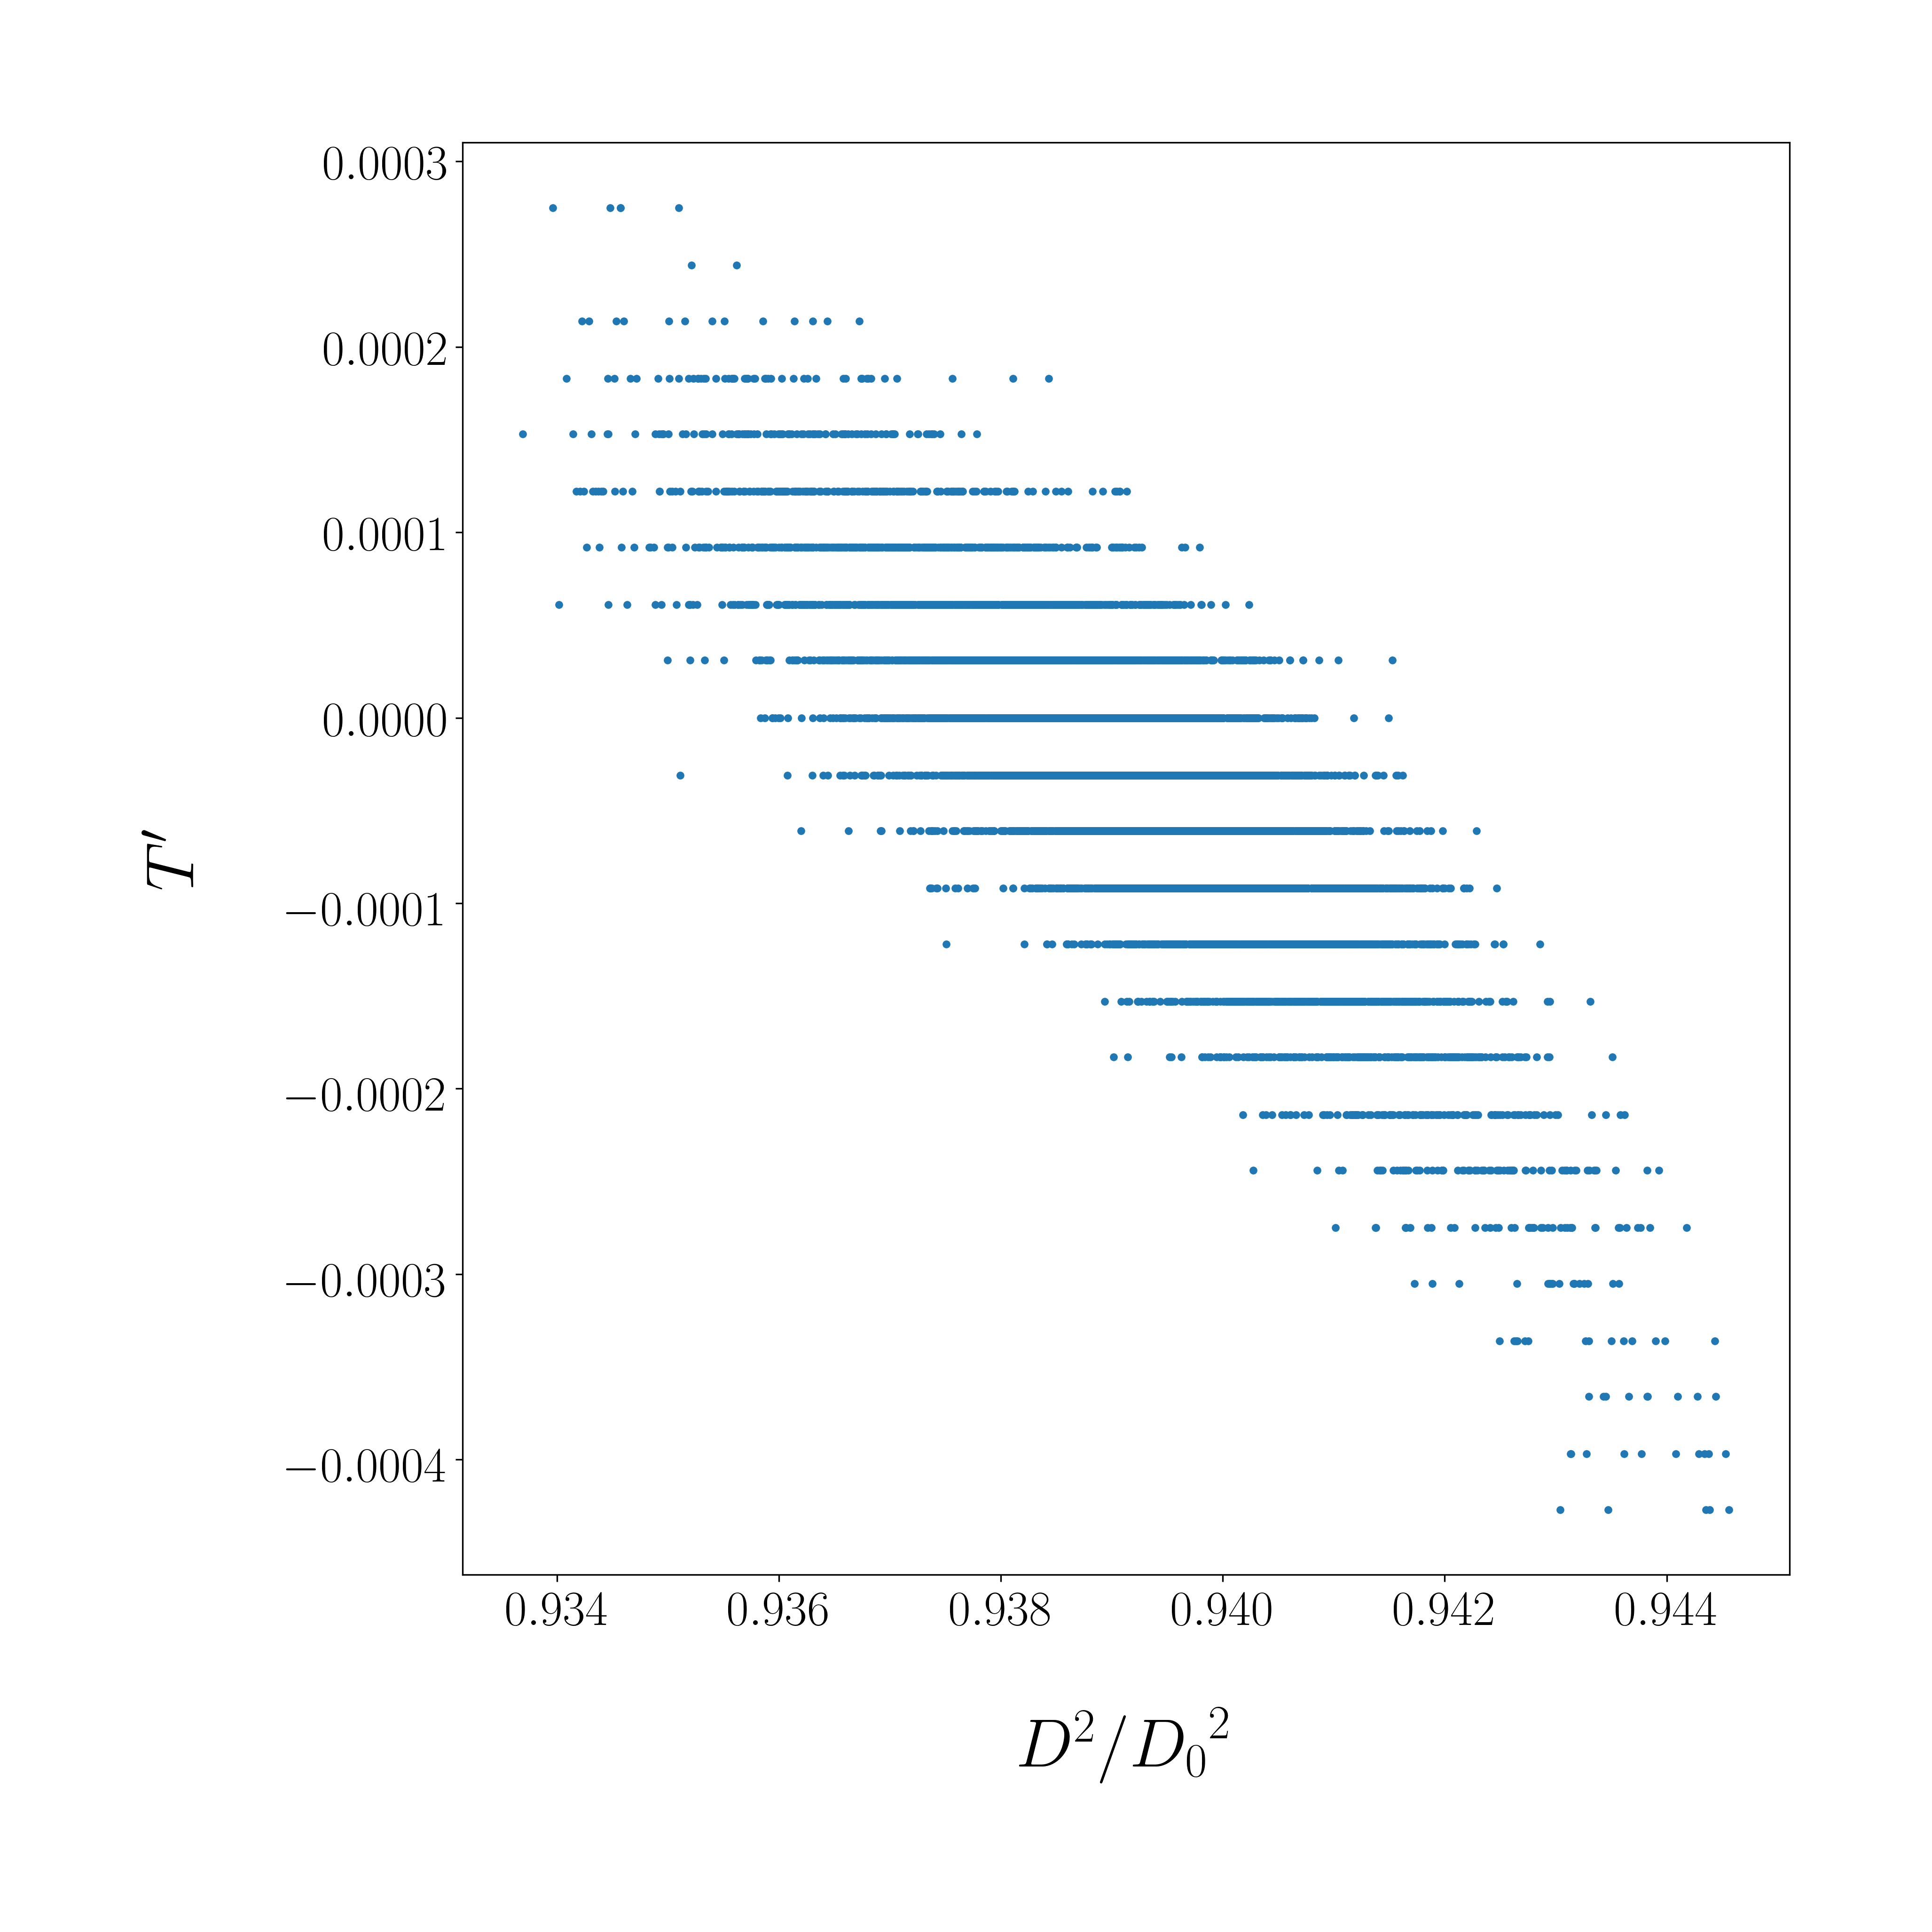
\includegraphics[width=0.7\textwidth]{./Diagrams/Temp_Mass_PDFs_timestep_80.png}
		\caption{}
	\end{subfigure}
\end{figure}
\begin{figure}\ContinuedFloat
	\centering
	\begin{subfigure}{\textwidth}
		\centering
		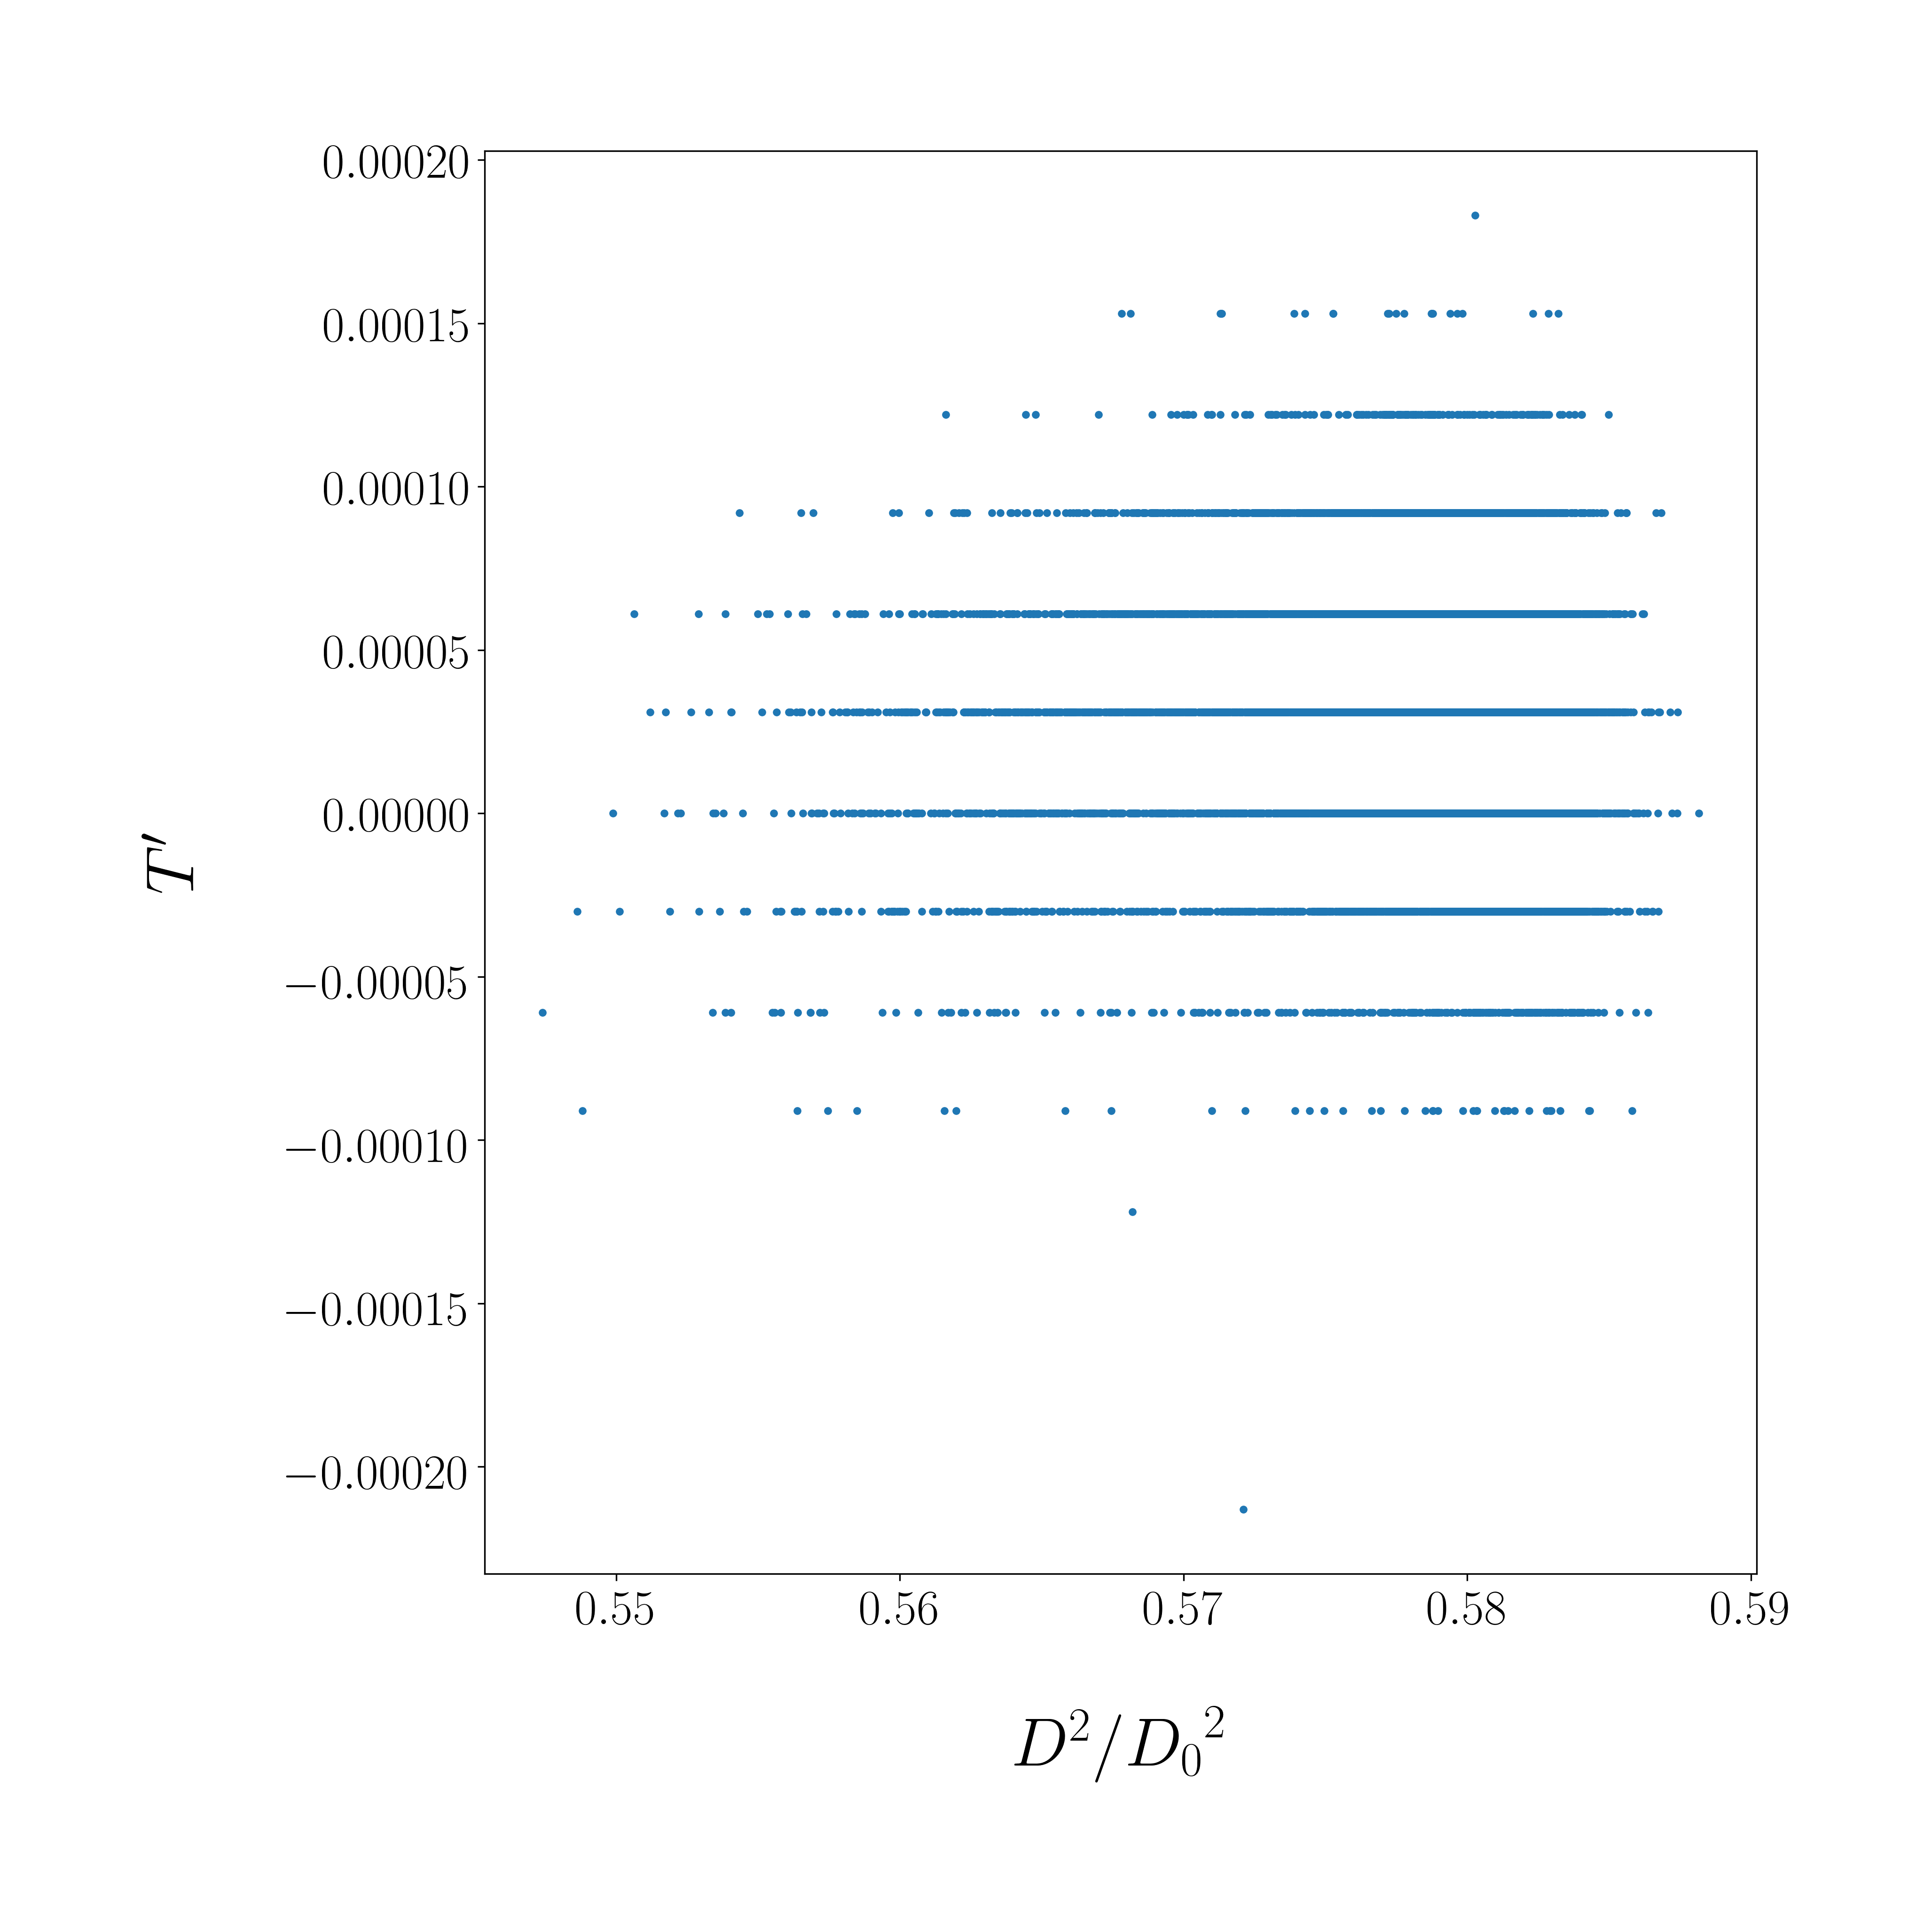
\includegraphics[width=0.7\textwidth]{./Diagrams/Temp_Mass_PDFs_timestep_800.png}
		\caption{}
\end{subfigure}
	\caption{$D^2/{D_0}^2$ against ${T_d}'$ at $1\tau_{d,0}$ (a), $10\tau_{d,0}$ (b) and $100\tau_{d,0}$ (c) into the simulation.}
	\label{fig:heat_mass_pdf}
\end{figure}
\subsection{Effect of Stokes Number on Heat Transfer}
The Stokes number will have some bearing on the heat and mass transfer of the droplets. This is because this will change how much the droplets follow the gas flow and therefore how much convective heat transfer there is.

For the simulation the settings in Table \ref{tab:sim_set} were used. However, instead of calculating $\mu_G$ using $T_R$ suitable values were chosen to give the required Stokes numbers. These values are given in Table \ref{tab:stk_nums}.
\begin{table}[H]
	\centering
	\begin{tabular}{|c c|}
		\hline
		\textbf{Kinematic Viscosity} & \textbf{Stokes Number} \\ \hline
		$2.2804\times 10^{-5}$ & 0.1 \\
		$2.2804\times 10^{-6}$ & 1.0 \\
		$2.2804\times 10^{-7}$ & 10.0 \\ \hline
	\end{tabular}
	\caption{Settings used to get different Stokes numbers.}
	\label{tab:stk_nums}
\end{table}

As mentioned previously the effect of the flow is to increase the deviation of droplet temperature and normalised droplet diameter. To compare results for different Stokes numbers the range between the maximum and minimum deviation for each timestep have been plotted in \ref{fig:t_prime_stks}.
\begin{figure}[H]
	\centering
	\begin{subfigure}{\textwidth}
		\centering
		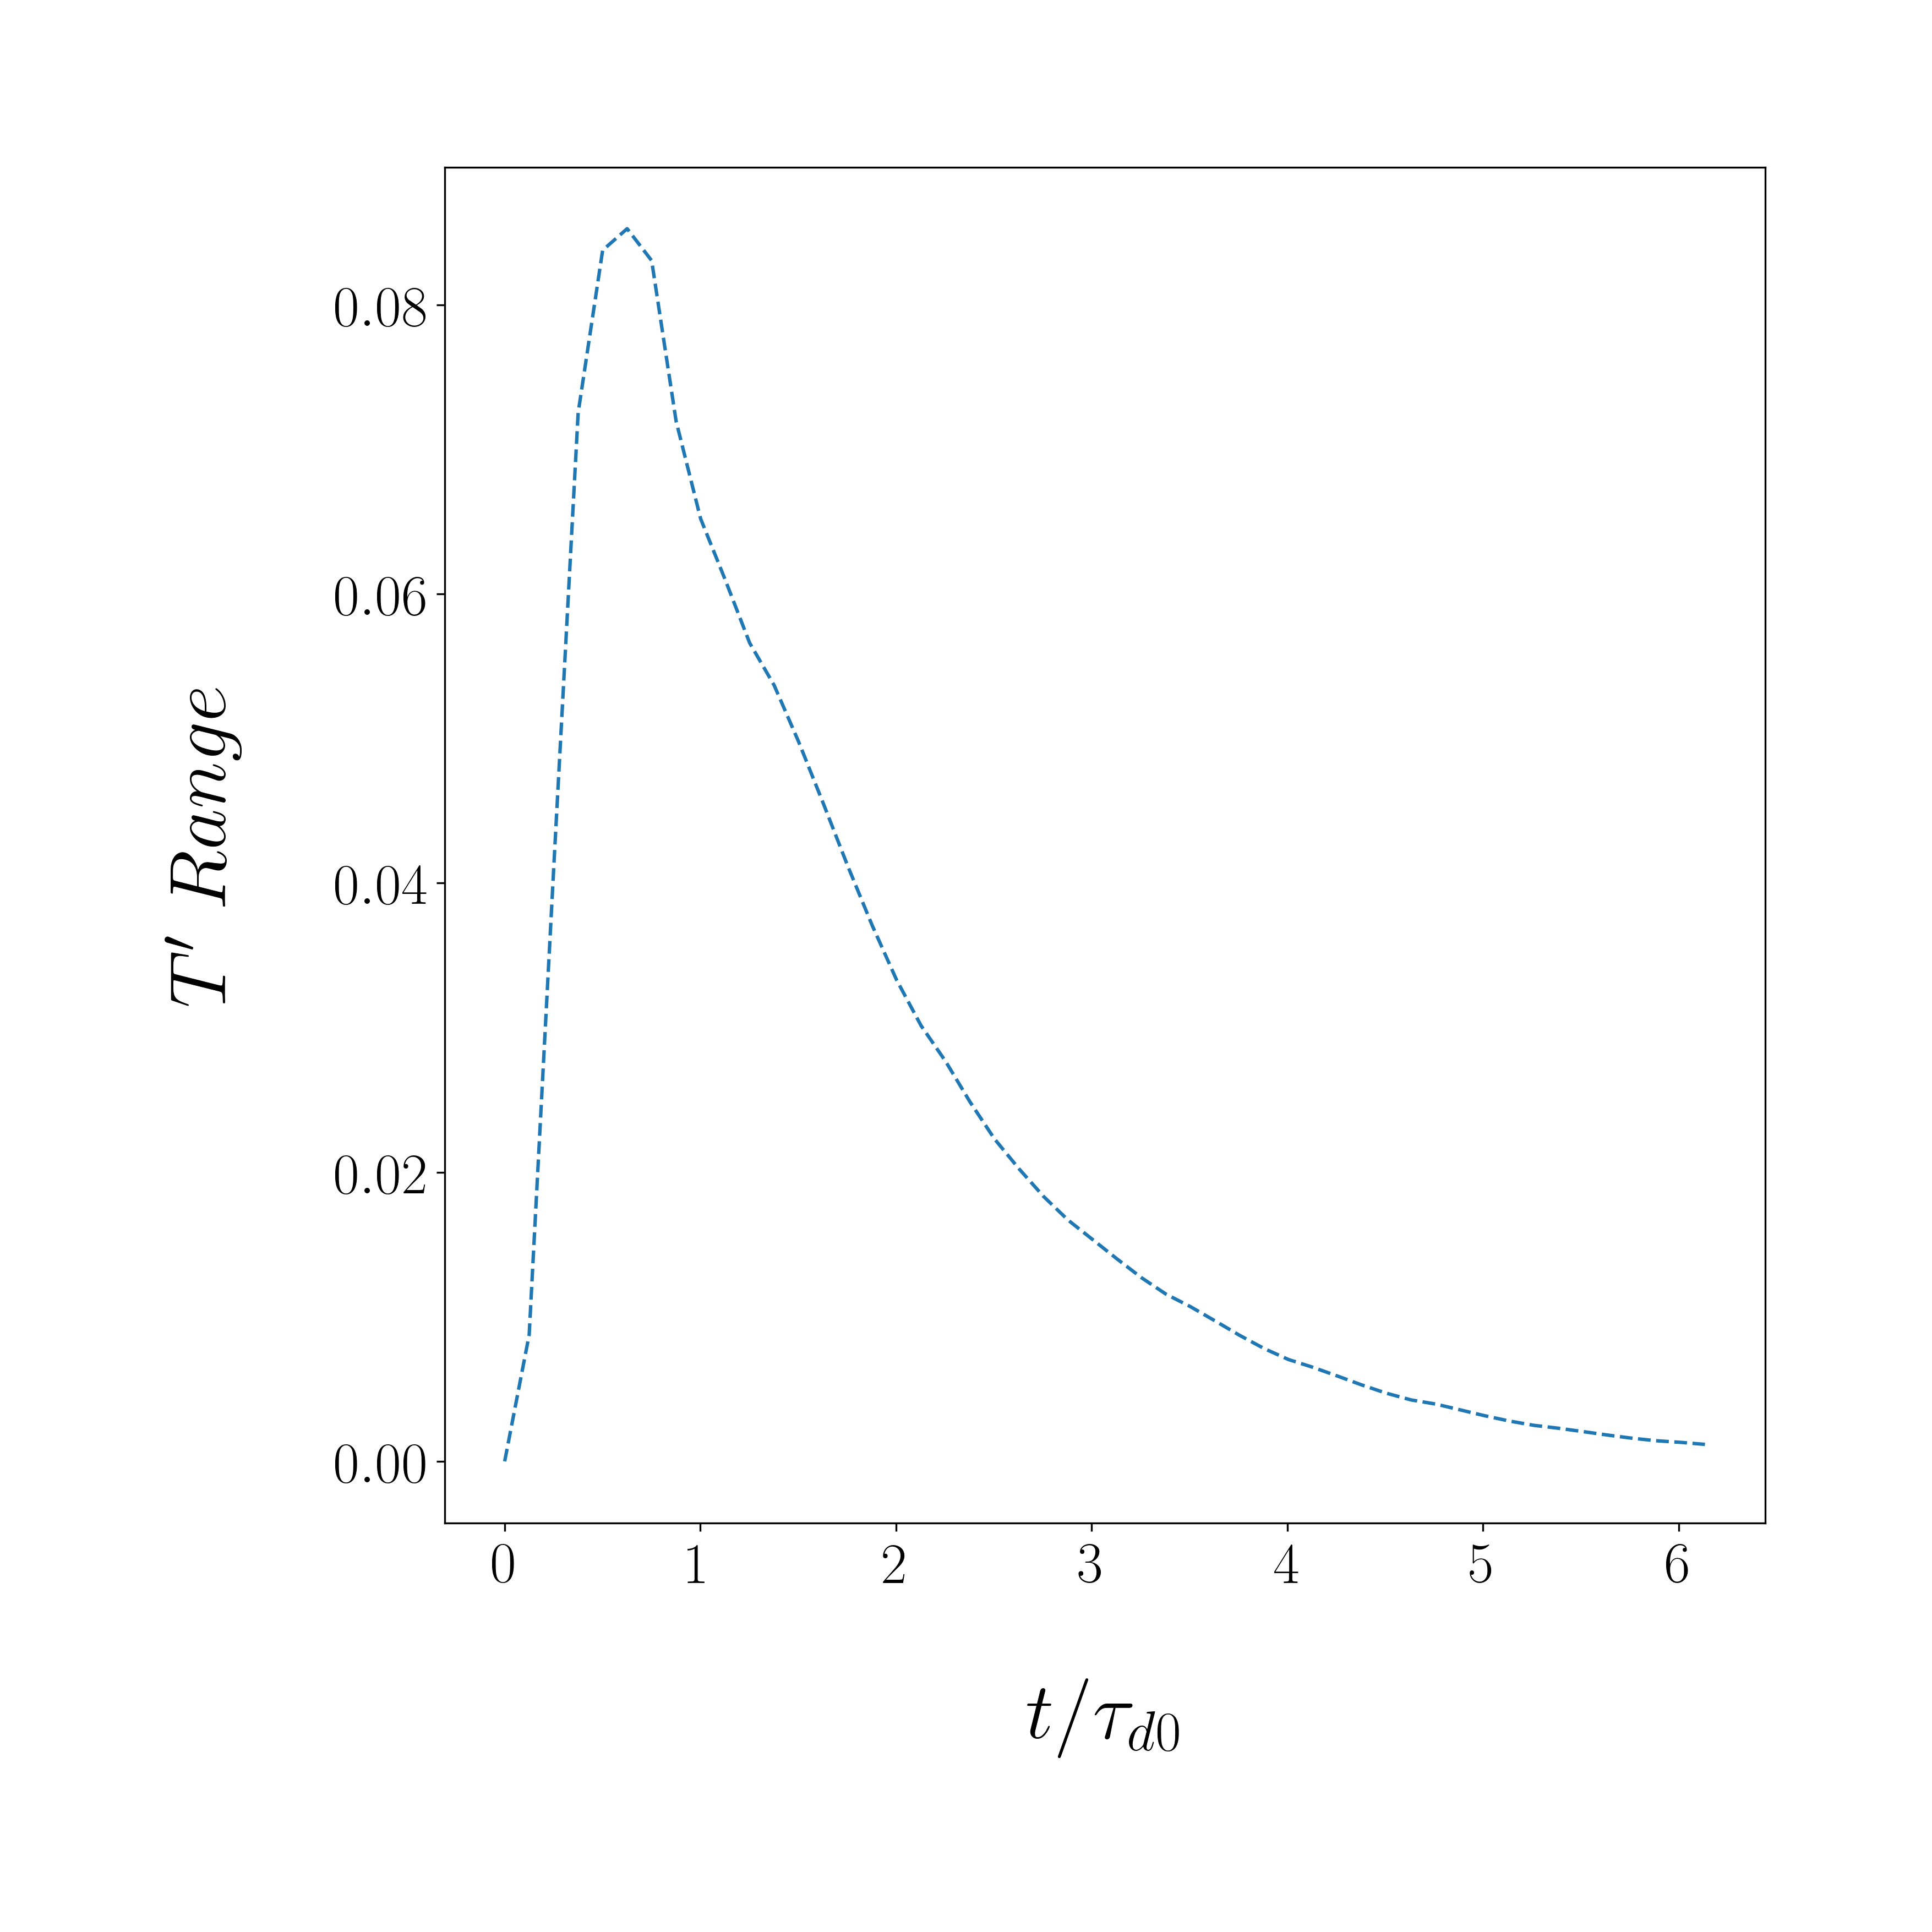
\includegraphics[width=0.7\textwidth]{./Diagrams/Temp_Deviation_0_1.png}
		\caption{}
	\end{subfigure}
\end{figure}
\begin{figure}\ContinuedFloat
	\centering
	\begin{subfigure}{\textwidth}
		\centering
		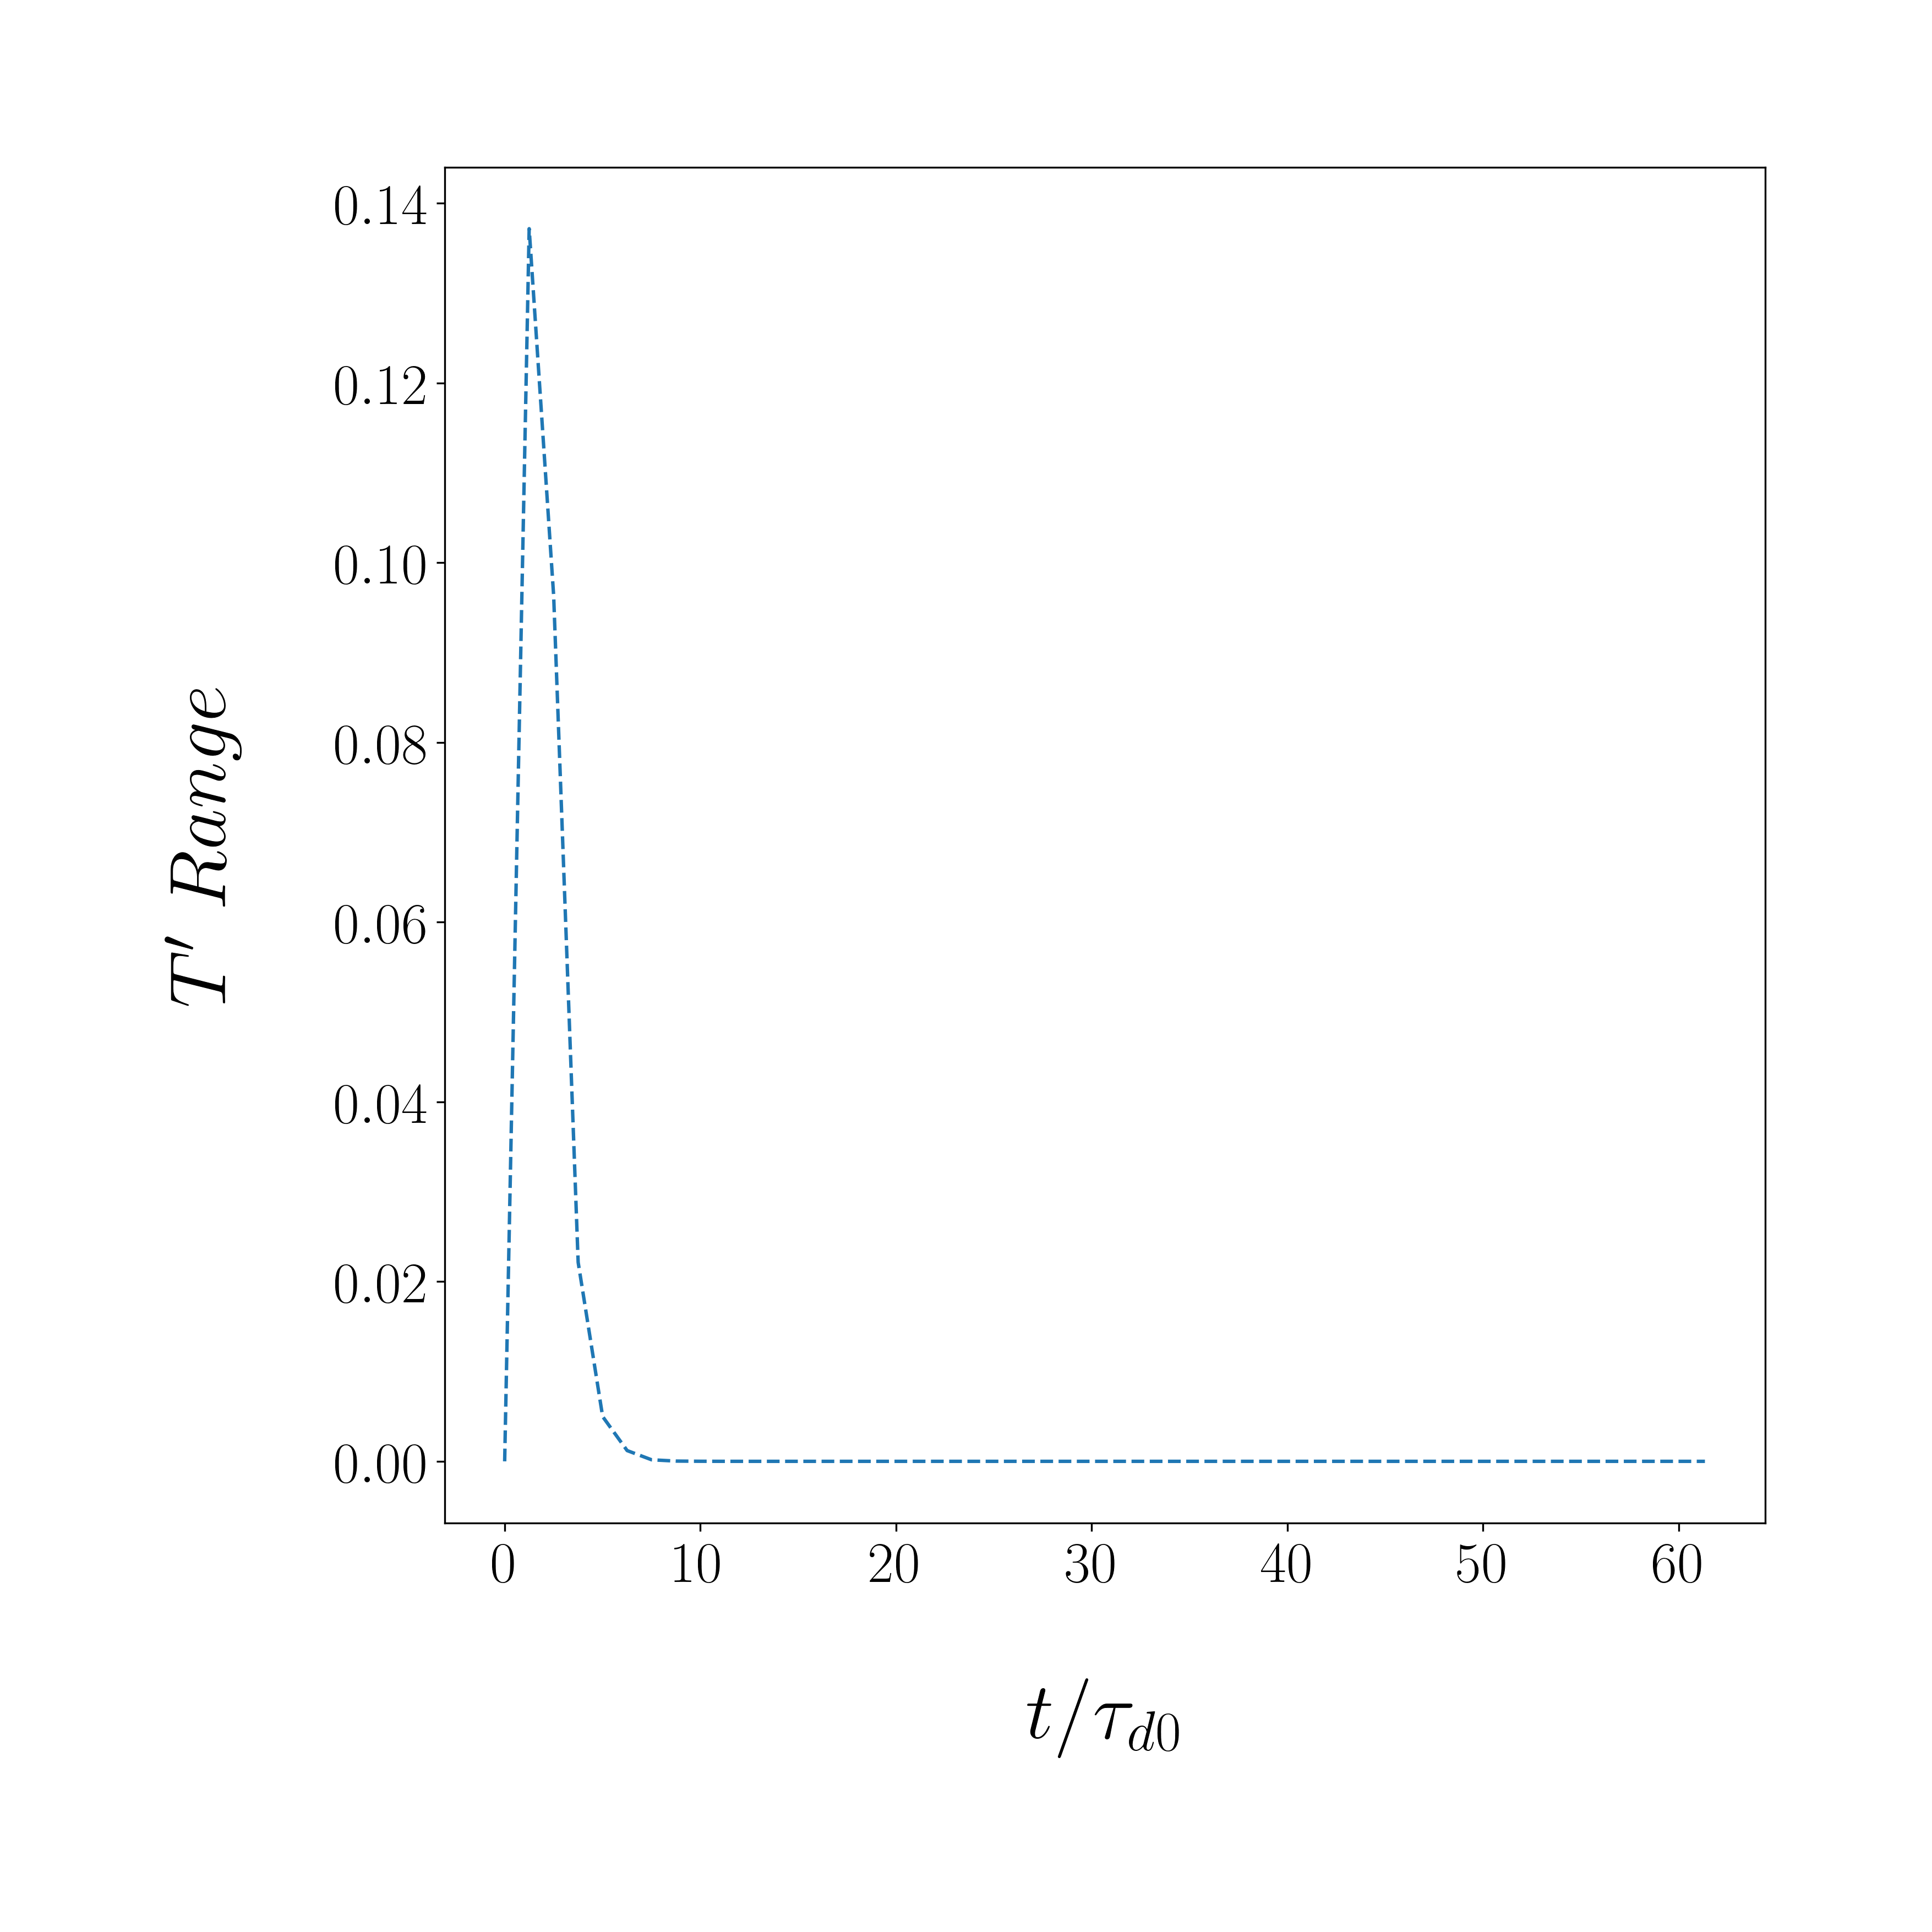
\includegraphics[width=0.7\textwidth]{./Diagrams/Temp_Deviation_1_0.png}
		\caption{}
	\end{subfigure}
\end{figure}
\begin{figure}\ContinuedFloat
	\centering
	\begin{subfigure}{\textwidth}
		\centering
		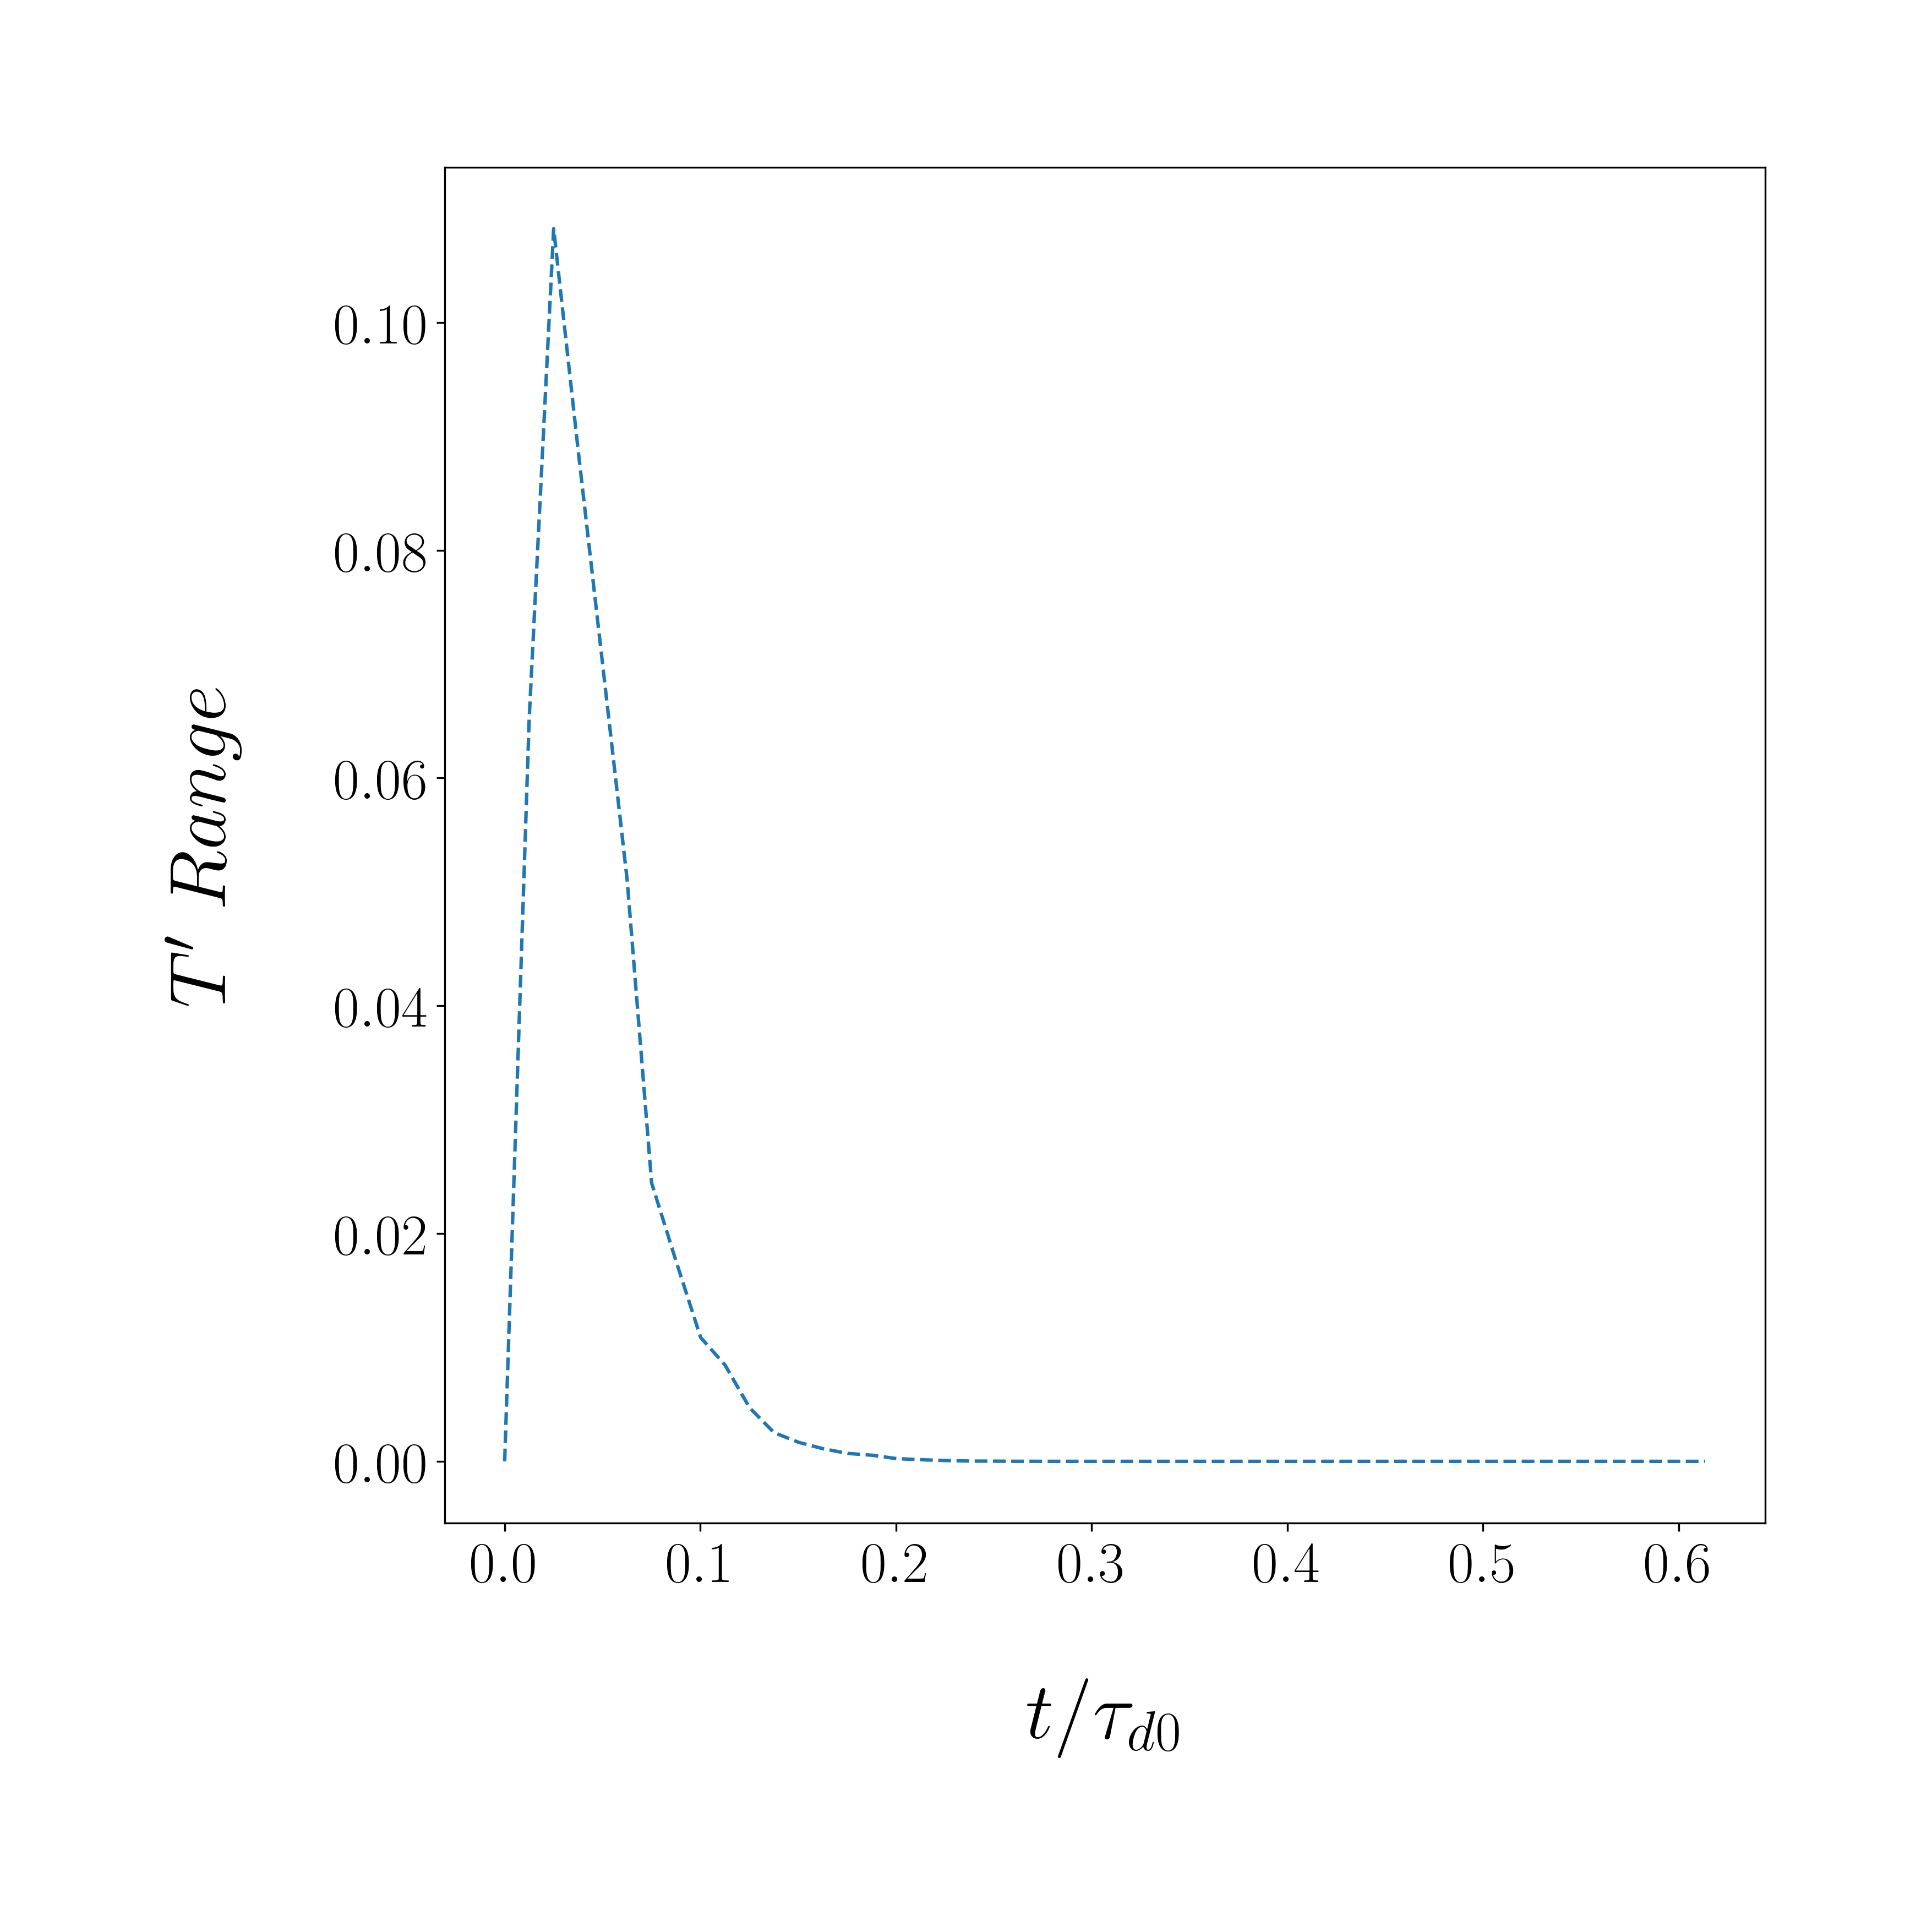
\includegraphics[width=0.7\textwidth]{./Diagrams/Temp_Deviation_10.png}
		\caption{}
	\end{subfigure}
	\caption{${T^\prime}'$ range for Stokes numbers of $0.1$ (a), $1.0$ (b) and $10$ (c)}
	\label{fig:t_prime_stks}
\end{figure}

Increasing the Stokes number has the effect of decreasing the range between the minimum and maximum $T^\prime$. Although this appears less pronounced for Stokes numbers between 0.1 and. This effect should be expected as for increasing Stokes numbers the less effect the fluid flow has on the droplet motion. Therefore, the difference in convective heat transfer between droplets will be less.
\end{document}
